\documentclass[aspectratio=169]{beamer}

\usepackage[utf8]{inputenc}
\usepackage{graphicx} % Allows including images
\usepackage{booktabs} % Allows the use of \toprule, \midrule and \bottomrule in tables
\usepackage{subfigure}
\usepackage{subfiles}
\usepackage{url}
\usepackage{amssymb}
\usepackage{amsmath}
\usepackage{xcolor,colortbl}
\usepackage{minted}
\usepackage{svg}
\usepackage[backend=bibtex,sorting=none]{biblatex}

\addbibresource{reference.bib} 

\definecolor{NJUPurple}{rgb}{0.41568, 0, 0.37255} 
\colorlet{LightNJUPurple}{white!60!NJUPurple}
\colorlet{SuperLightNJUPurple}{white!90!NJUPurple}

% \hypersetup{colorlinks,linkcolor=,urlcolor=LightNJUPurple,pdfborderstyle={/S/U/W 1}}


\usecolortheme[named=NJUPurple]{structure}
\setmintedinline{bgcolor={}} 
%Information to be included in the title page:
\title{How to Debug Your Python Program}
\author{Shengyi Jiang, Qinlin Chen, Yicheng Huang, \\ Zhiqi Chen \& Zhehao Lin}
\date{\today}

%Logo in every slide
\logo{%
  \makebox[0.98\paperwidth]{
    \href{https://www.nju.edu.cn}{
\includegraphics[height=0.75cm,keepaspectratio]{logos/nju_logo.jpg}}
    \hfill%
    \href{https://cs.nju.edu.cn}{
\includegraphics[height=1.0cm,keepaspectratio]{logos/njucs_logo.jpg}}%
  }
}

\setbeamertemplate{blocks}[rounded][shadow=true]
\setbeamercolor{block title}{fg=white,bg=LightNJUPurple}
\setbeamercolor{block body}{fg=black,bg=SuperLightNJUPurple}
\setbeamerfont{title}{size=\huge}
% \setbeamerfont{author}hug

\makeatletter
\setbeamertemplate{title page}{%
  \vbox{}
  \vfill
  \vskip2cm%<- added
  \begingroup
    \centering
    \begin{beamercolorbox}[sep=8pt,center]{title}
      \usebeamerfont{title}\inserttitle\par%
      \ifx\insertsubtitle\@empty%
      \else%
        \vskip0.25em%
        {\usebeamerfont{subtitle}\usebeamercolor[fg]{subtitle}\insertsubtitle\par}%
      \fi%     
    \end{beamercolorbox}%
    \vskip1em\par
    \vfill%<- added
    \begin{beamercolorbox}[sep=8pt,center]{author}
      \usebeamerfont{author}\insertauthor
    \end{beamercolorbox}
    \vskip-0.2cm%<- changed
    \begin{beamercolorbox}[sep=8pt,center]{institute}
      \usebeamerfont{institute}\insertinstitute
    \end{beamercolorbox}
    \vfill%<- added
    \begin{beamercolorbox}[sep=8pt,center]{date}
      \usebeamerfont{date}\insertdate
    \end{beamercolorbox}%
    \vskip0.5cm%<- changed
  \endgroup
%  \vfill%<- removed
}
\makeatother


\AtBeginSection[]
{
  \begin{frame}
    \frametitle{Table of Contents}
  \tableofcontents[
        currentsection,
        currentsubsection,
        subsectionstyle=show/show/hide,
        sectionstyle=show/shaded
    ]
  \end{frame}
}


% shape, colour of item, nested item bullets in itemize only
\setbeamertemplate{itemize item}[circle] \setbeamercolor{itemize item}{bg=blue}
\setbeamertemplate{itemize subitem}[circle] \setbeamercolor{itemize subitem}{fg=LightNJUPurple}
\setbeamertemplate{itemize subsubitem}[triangle] \setbeamercolor{itemize subsubitem}{fg=LightNJUPurple}
% \setbeamertemplate{itemize/enumerate body begin}{\normalsize}
% \setbeamertemplate{itemize/enumerate subbody begin}{\normalsize}
% font size of nested and nested-within-nested bulltes in both itemize and enumerate
% options are \tiny, \small, \scriptsize, \normalsize, \footnotesize, \large, \Large, \LARGE, \huge and \Huge


\setbeamerfont{itemize/enumerate subbody}{size=\scriptsize} 
\setbeamerfont{itemize/enumerate subsubbody}{size=\scriptsize}


\newenvironment{splitframe}[5]
%[1] ==> 1 parameter passed through {}
%[2] ==> 2 parameters passed through {}{}
%[4] ==> 4 parameters passed through {}{}{}{}
    {
    \begin{frame}{#3}
    \begin{columns}
    \column{#1\linewidth}
    \centering
    #4
    \column{#2\linewidth}
    \centering
    #5
    \end{columns}
    \centering
    \vspace{\baselineskip} % adds one line space
    }
    %Inside the first pair of braces (ABOVE) is set what your new environment will do before the text within, then inside the second pair of braces (BELOW) declare what your new environment will do after the text. Note second pair can be empty braces too.
    {
    \end{frame}
    }

\begin{document}

\frame{\titlepage}

% no hyperlinks in logos except for titlepage
\logo{%
  \makebox[0.98\paperwidth]{
    
\includegraphics[height=0.75cm,keepaspectratio]{logos/nju_logo.jpg}
    \hfill%
    
\includegraphics[height=1.0cm,keepaspectratio]{logos/njucs_logo.jpg}%
  }
}

\begin{frame}
\frametitle{Table of Contents}
\tableofcontents[hidesubsections]
\end{frame}

\section{What can errors tell you}

\begin{frame}
\frametitle{What can errors tell you}
Most Python errors are self-explanatory. 

\begin{itemize}
\item \textbf{SyntaxError}:	Improper syntax (e.g. a missing colon or unpaired parentheses/quotes);
\item \textbf{IndentationError}: Improper indentation (e.g. inconsistent indentation of a function body);
\item \textbf{TypeError}: Attempted operation on incompatible types (e.g. trying to add a function and a number) or function call with the wrong number of arguments;
\item \textbf{ZeroDivisionError}: Attempted division by zero;
\end{itemize}

\end{frame}

\begin{frame}
\frametitle{Cherish Such Kind Error Indications}
\begin{figure}
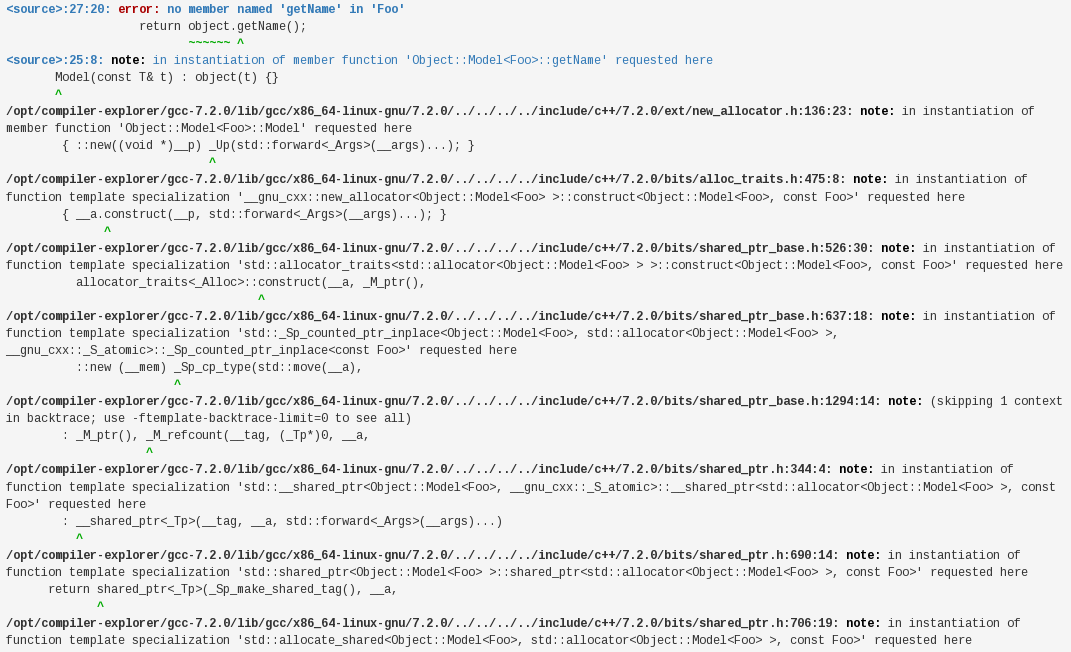
\includegraphics[width=0.6\linewidth]{./imgs/errorClang.png}
\caption{A Typical C++ Template Error}
\end{figure}
\end{frame}

\begin{frame}[fragile]
\frametitle{Do Not Be Afraid of Seeing Errors}
\begin{columns}
\begin{column}{0.3\textwidth}
\begin{minted}[escapeinside=||]{python}
def a_plus_abs_b(a, b): 
    if b >= 0:
        h = a + b
    else:
        h = a - b
    |\colorbox{white!50!red}{return h(a, b)}|
\end{minted}
\end{column}
\begin{column}{0.7\textwidth}  
\begin{center}
\begin{minted}[escapeinside=||]{text}
  File "*", line 23, in <module>
    a_plus_abs_b(2, 3)
  File "*", line 21, in a_plus_abs_b
    return h(a, b)
TypeError: 'int' object is not callable
\end{minted}
\end{center}
The error message indicates the location (File and Line No.) and type (TypeError) of your error. 
The text \mintinline{text}{'int' object is not callable} also tells you that \mintinline{text}{h} should be a function.
\end{column}
\end{columns}

\vspace{5mm}
\textbf{Note}: You can Baidu or Google the error if you do not understand its meaning.
\end{frame}


\begin{frame}
\frametitle{Errors are not enough}

\vspace{1.5cm}
Sometimes, the program crashes long after your actual error (or does not crash but gives you a wrong answer). In such cases, errors may not provide useful information and sometimes lead you to a wrong direction.
\vfill
\href{https://www.zhihu.com/question/21747929}{\underline{Interesting bugs in real life.}}

\end{frame}

\section{Debug using debugger}
\label{sec:debugger}
\begin{frame}
\frametitle{Debug using debugger}

\begin{block}{Debugger}
A debugger or debugging tool is a computer program used to test and debug other programs (the "target" program).  Typical debugging facilities include the ability to
\begin{itemize}
    \item run or halt the target program at specific points
    \item display frame contents
    \item modify frame contents
\end{itemize}
\end{block}

Notes: We will show examples about using debugger in PyCharm(\href{https://www.jetbrains.com/help/pycharm/debugging-code.html}{\underline{docs}}). Things are similar in VSCode, so you may find the usage yourself. You can also try to use debugger in terminal (\href{https://docs.python.org/3.8/library/pdb.html}{\underline{docs for \mintinline{text}{pdb}}}).


\end{frame}


\begin{frame}
\frametitle{Add a configuration in PyCharm}
PyCharm does not support debugging a \mintinline{text}{doctest} directly (You can try to debug a doctest and see what will happen). We need to add a new Python configuration for debugging. The general process is similar to adding a \mintinline{text}{doctest} configuration.
\end{frame}

\begin{frame}
\frametitle{Add a configuration in PyCharm}

\begin{figure}
    \centering
    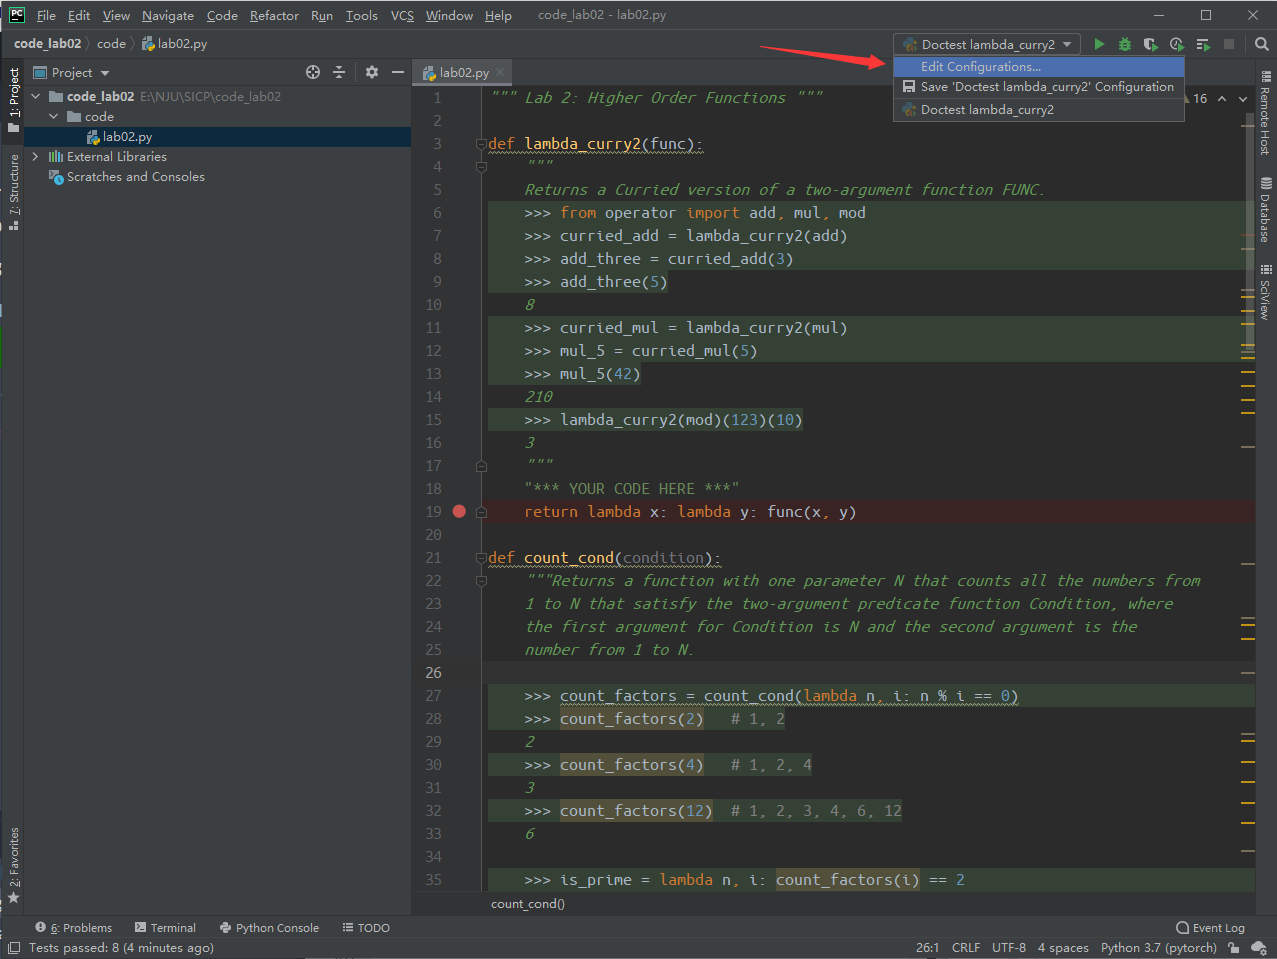
\includegraphics[width=0.5\linewidth]{./imgs/config1.png}
    \caption{Click \mintinline{text}{Edit Configurations}}
    \label{fig:config}
\end{figure}
\end{frame}

\begin{frame}
\frametitle{Add a configuration in PyCharm}

\begin{figure}
    \footnotesize
    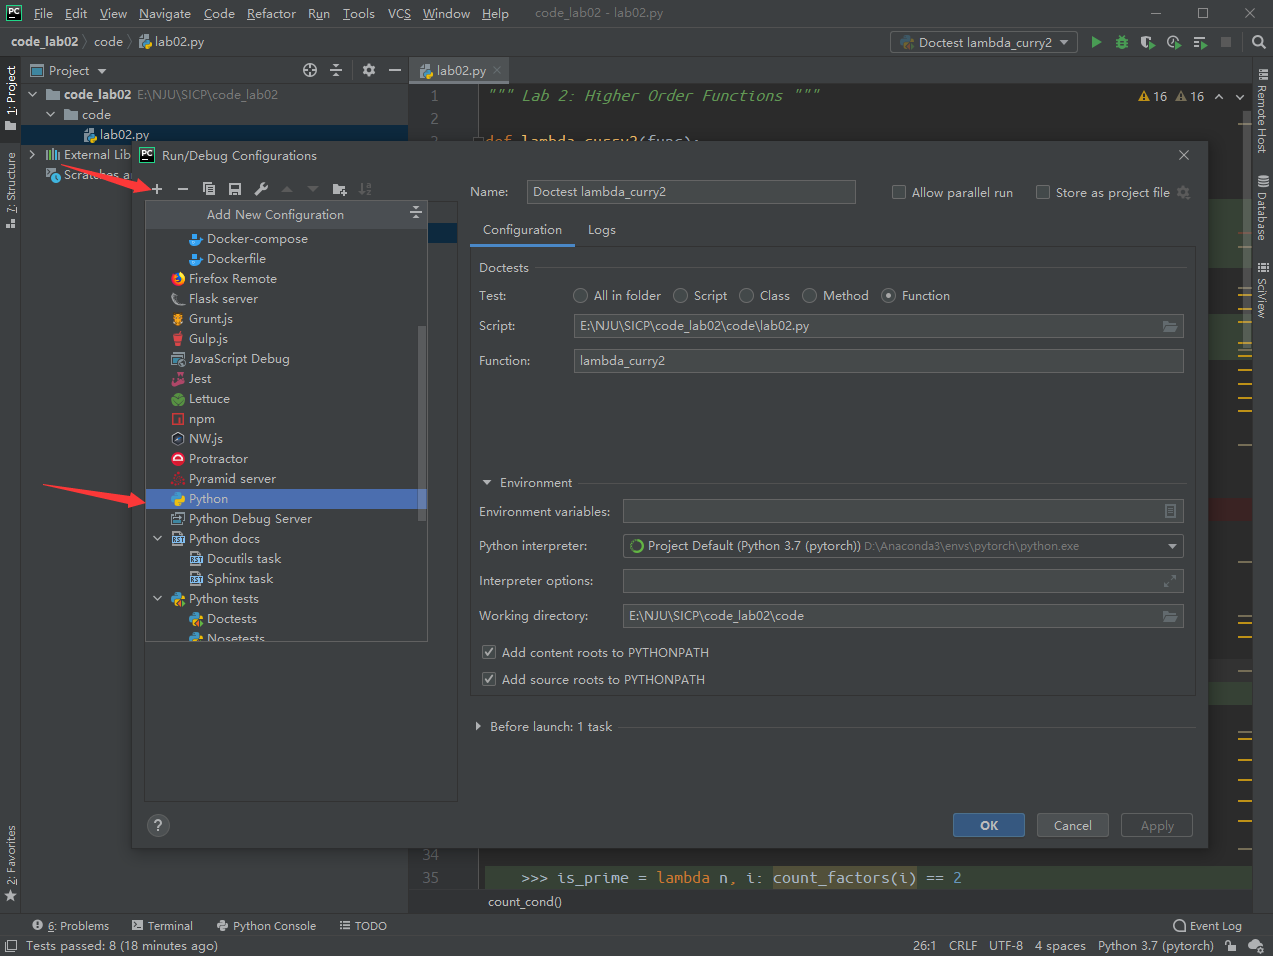
\includegraphics[width=0.5\linewidth]{./imgs/config2.png}
    \caption{Click \mintinline{text}{+} and choose \mintinline{text}{Python}}
    \label{fig:config2}
\end{figure}
\end{frame}

\begin{frame}
\frametitle{Add a configuration in PyCharm}

\begin{figure}
    \centering
    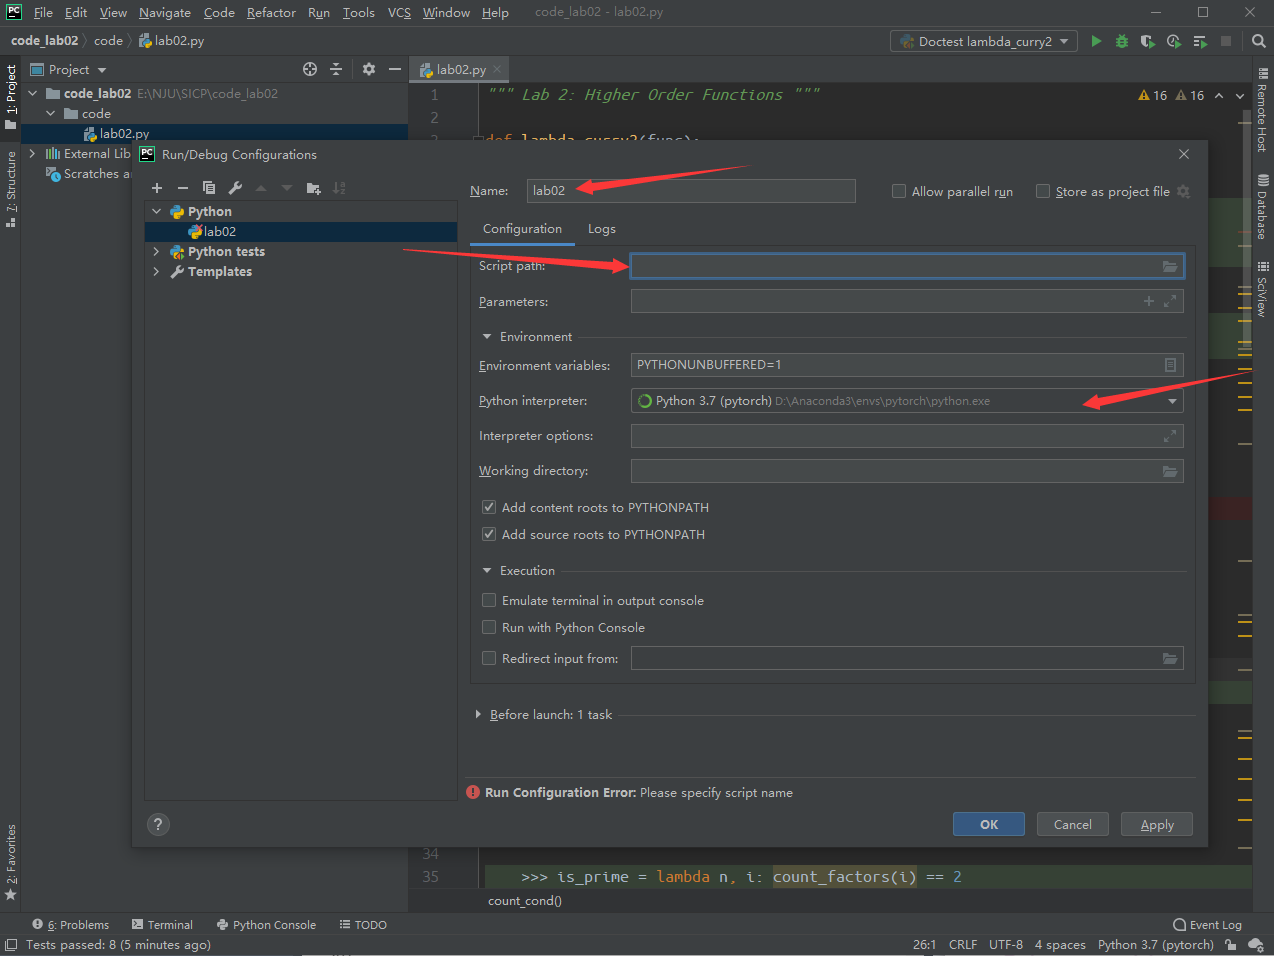
\includegraphics[width=0.45\linewidth]{./imgs/config3.png}
    \caption{Change \mintinline{text}{Name, Scripts path, Python interpreter}.}
    \label{fig:config3}
\end{figure}

\vspace{-5mm}
\small{You can use any  \mintinline{text}{Name}, but \mintinline{text}{Scripts path, Python interpreter} must be correct.}

\end{frame}

\begin{frame}
\begin{figure}
    \centering
    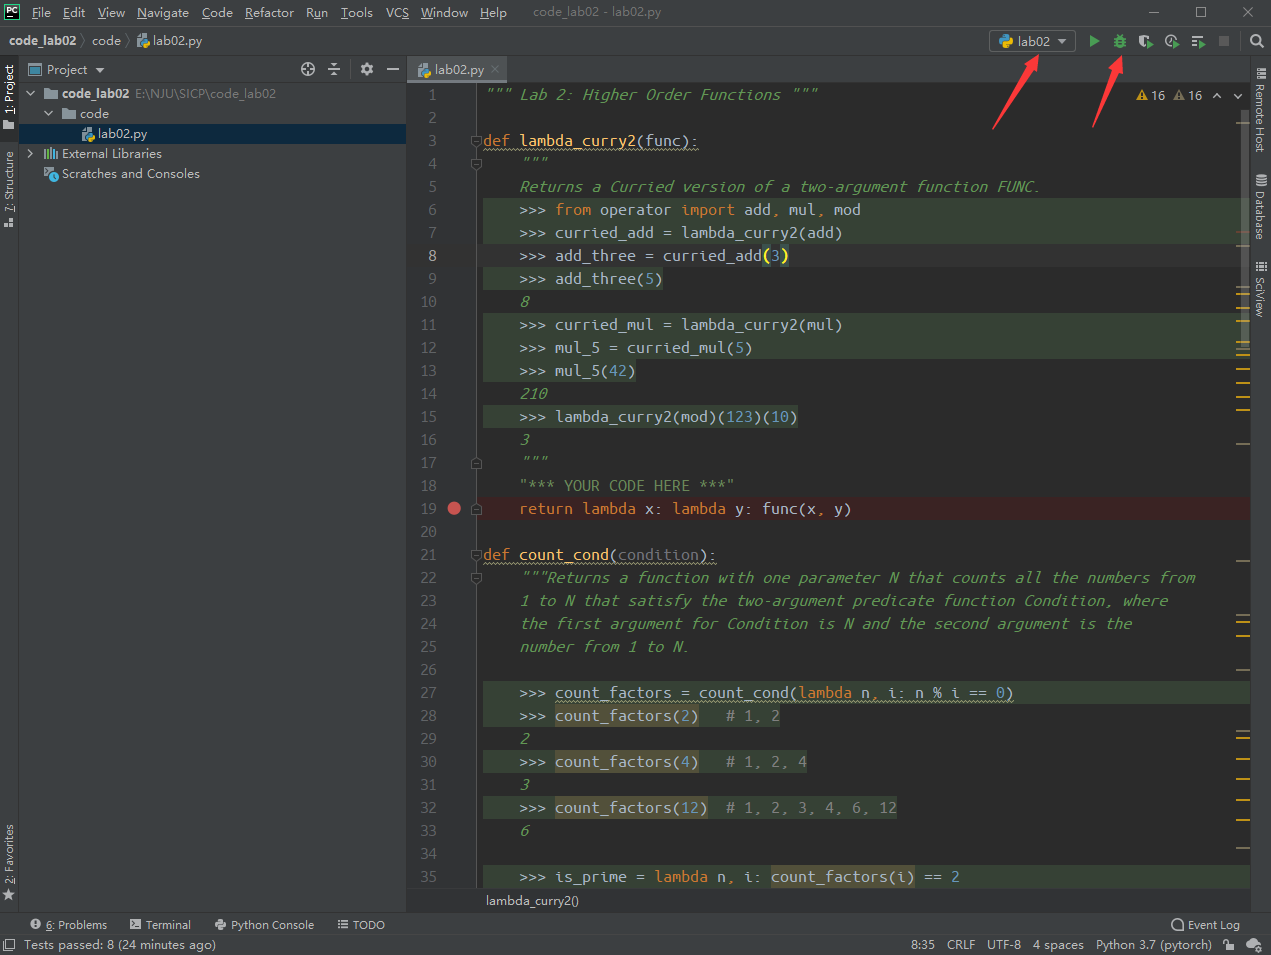
\includegraphics[width=0.5\linewidth]{./imgs/run_debugger.png}
    \caption{Select the configuration you just created and click \mintinline{text}{Debug} button}
    \label{fig:config3}
\end{figure}
\end{frame}

\begin{frame}
\vspace{20mm}
\begin{center}
Hmm, nothings happens. Why?

You do not actually CALL any functions in the script.
\end{center}
\vspace{25mm}
Note: \mintinline{text}{doctest} does the function call automatically to check if your function output matches the expected one.
\end{frame}

\begin{frame}
\frametitle{Make a Function Call}
Explicitly add a function call to the function you have implemented. You can choose \mintinline{text}{doctest} examples or design some new cases as function inputs.
\begin{figure}
    \centering
    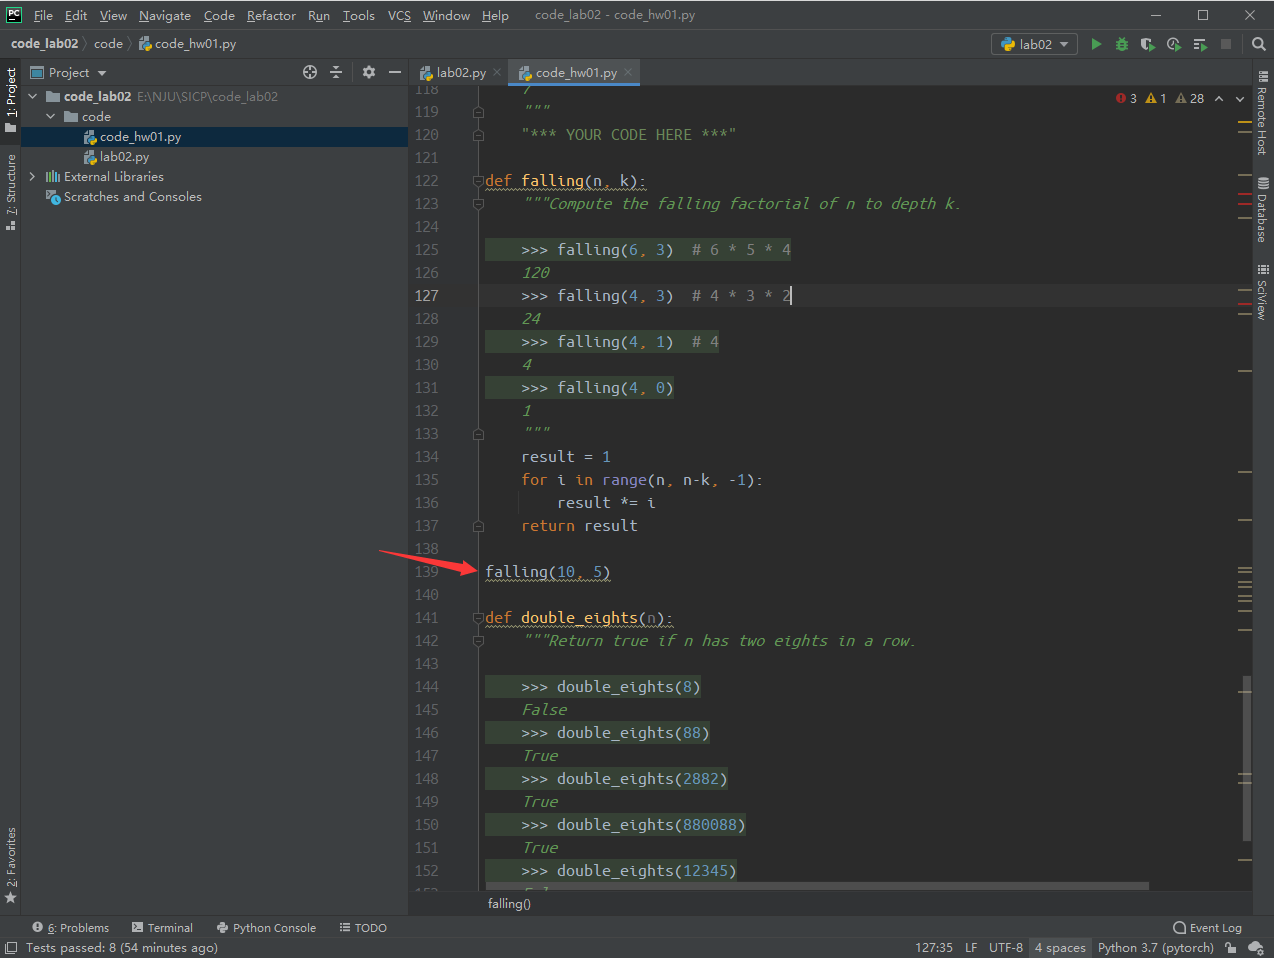
\includegraphics[width=0.5\linewidth]{./imgs/add_func_call.png}
    \label{fig:add_func_call}
\end{figure}
\end{frame}


\begin{frame}
\frametitle{Add a Breakpoint}
\begin{figure}
    \centering
    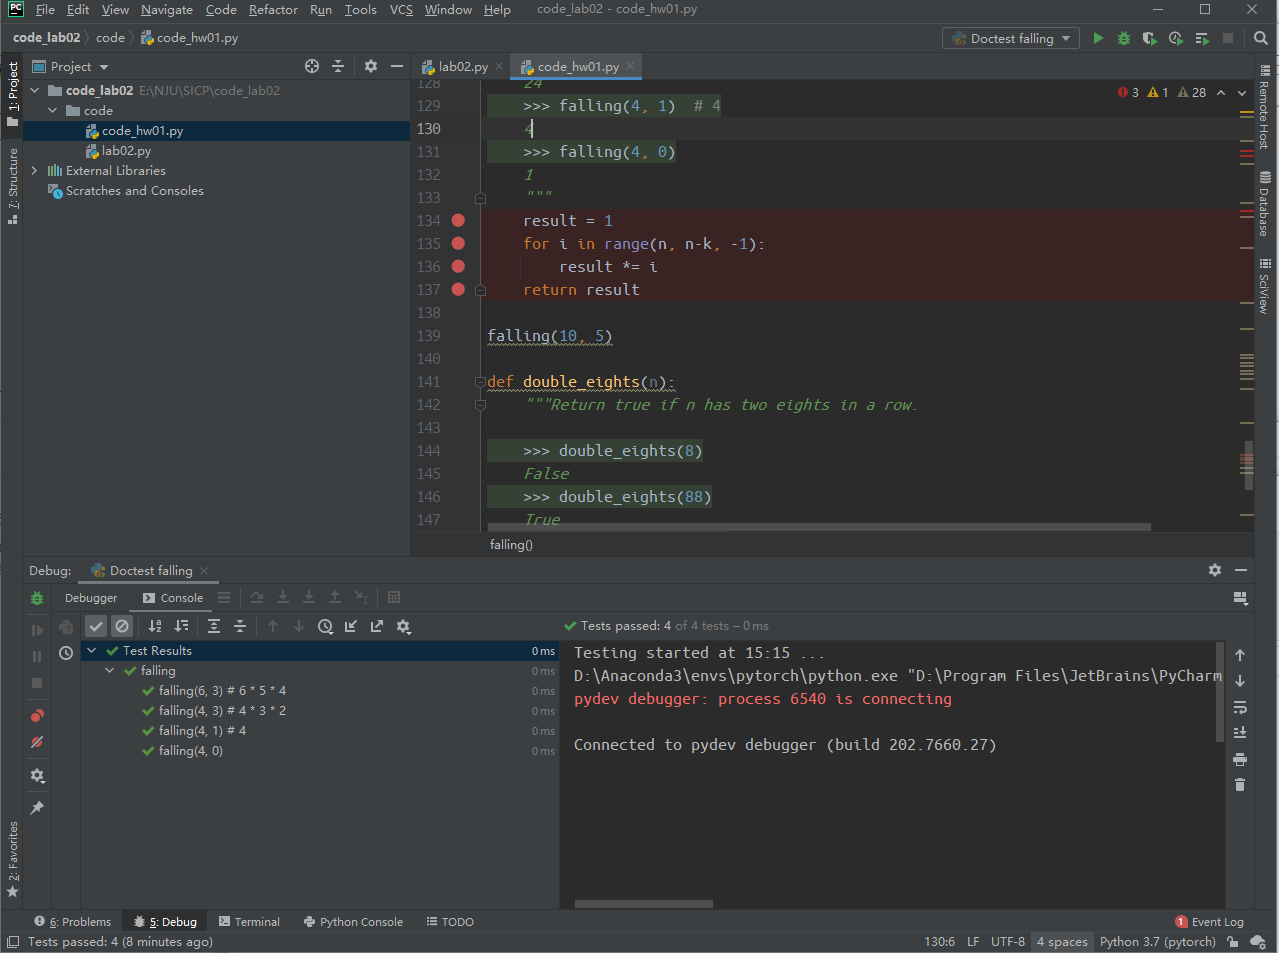
\includegraphics[width=0.45\linewidth]{./imgs/breakpoint.png}
    \caption{Click the space right to the line no. to add a breakpoint. Click the circle to cancel it.}
    \label{fig:breakpoint}
\end{figure}
\vspace{-5mm}
\small{\textbf{Breakpoint}: debugger will halt the program when reaching a breakpoint.}
\end{frame}


% \begin{frame}
% \frametitle{Control the debugging process}

% \begin{columns}
% \begin{column}{0.5\textwidth}
% \begin{figure}
%     \centering
%     \includesvg[width=0.45\linewidth]{./imgs/icons.actions.traceOver.svg}
%     \caption{Different options to control the debugging.}
%     \label{fig:breakpoint}
% \end{figure}
% \end{column}
% \begin{column}{0.5\textwidth}
% \begin{figure}
%     \centering
%     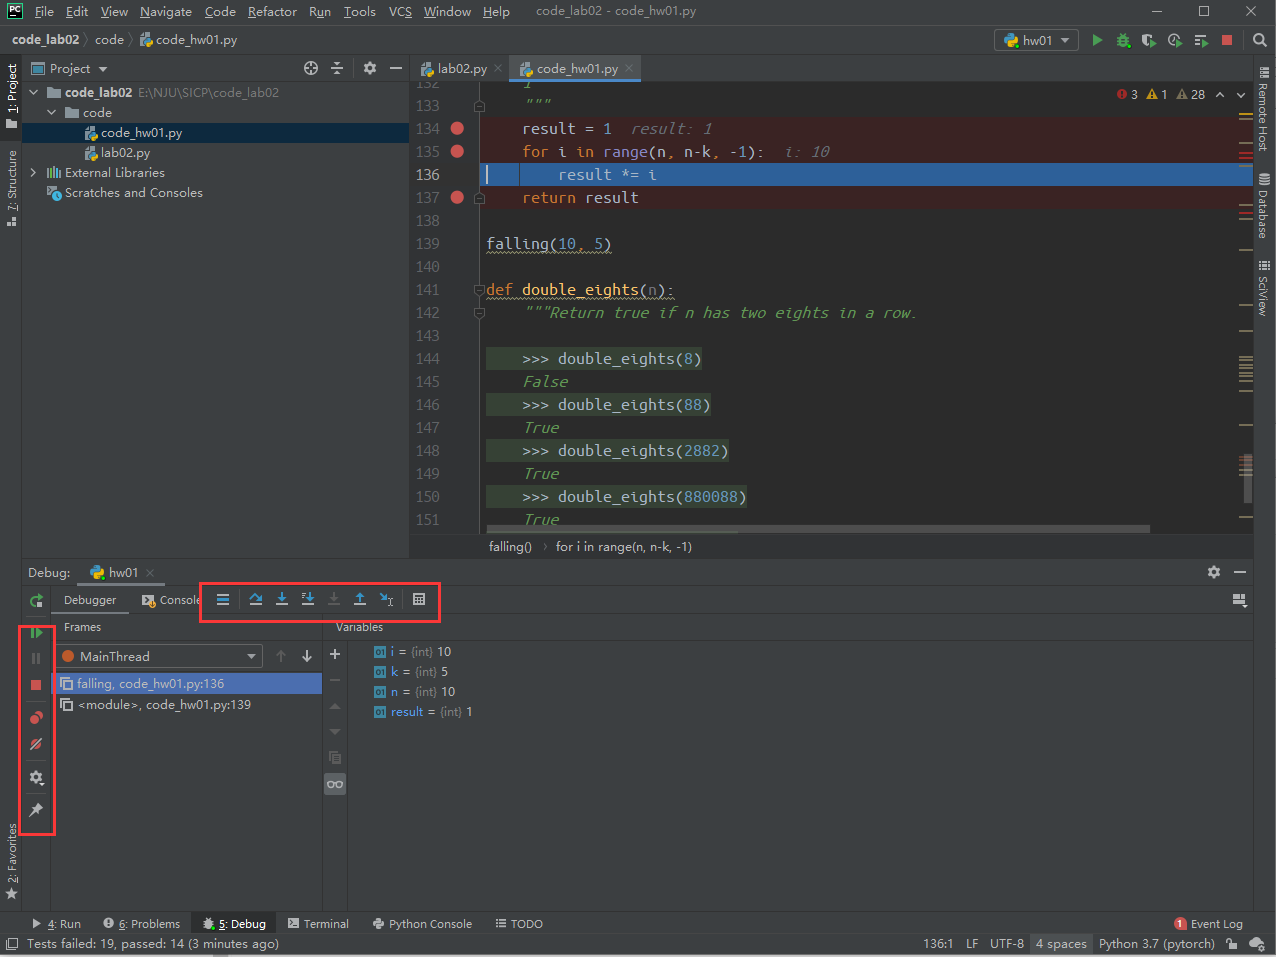
\includegraphics[width=0.45\linewidth]{./imgs/step.png}
%     \caption{Different options to control the debugging.}
%     \label{fig:breakpoint}
% \end{figure}
% \end{column}
% \end{columns}


\begin{frame}
\frametitle{Control the debugging process}
{\footnotesize
\begin{itemize}
    \item \includesvg{./imgs/icons.actions.resume.svg} {Resume: Resume a debug session (stop at the next breakpoint).}
    \item \includesvg{./imgs/icons.actions.pause.svg}  \ \  Pause: Pause the code and show the current execution point.
    \item \includesvg{./imgs/icons.actions.traceOver.svg} {Step Over: Steps over the current line of code and takes you to the next line even if the highlighted line has method calls in it.}
    \item \includesvg{./imgs/icons.actions.traceInto.svg} Step Into: Steps into the method to show what happens inside it.
    \item \includesvg{./imgs/python.icons.com.jetbrains.python.debug.StepIntoMyCode.svg} Step Into My Code: Same as above, but ignores code of thirdparty libraries.
    \item 
\includegraphics[width=1.1em]{./imgs/icons.debugger.actions.force_step_into.png} Force Step Into:     Steps in the method even if this method is skipped by the regular Step Into.
    \item \includesvg{./imgs/icons.actions.stepOut.svg} Step Out: Steps out of the current method and takes you to the caller method.
    \item \includesvg{./imgs/icons.actions.runToCursor.svg} Run To Cursor: Continues the execution until the position of the caret is reached.
\end{itemize}}
\end{frame}


\begin{frame}
\frametitle{Make Debugging Great Again}
Select the configuration you just created and click \mintinline{text}{Debug} button AGAIN.
\vfill
\begin{center}
    \textbf{What can we get from debugging?}
    \vspace{5mm}
\end{center}
\end{frame}
\begin{frame}
\frametitle{Variable Value}
\begin{figure}
    \centering
    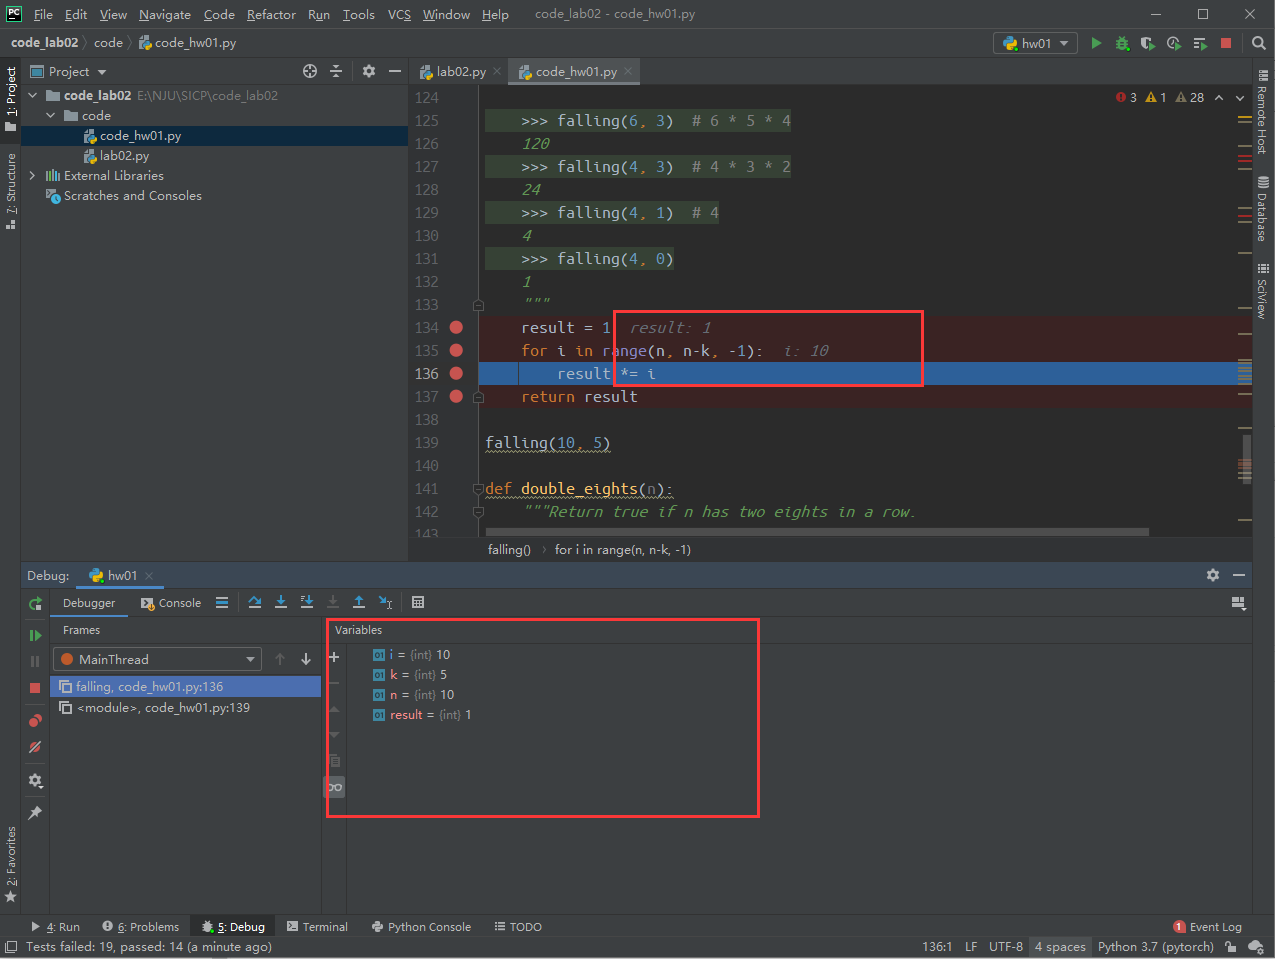
\includegraphics[width=0.45\linewidth]{./imgs/var_value.png}
    \caption{PyCharm will display values of variables in selected regions.}
    \label{fig:breakpoint}
\end{figure}
\vspace{-5mm}
\end{frame}

\begin{frame}
\frametitle{Call Stack}
\begin{figure}
    \centering
    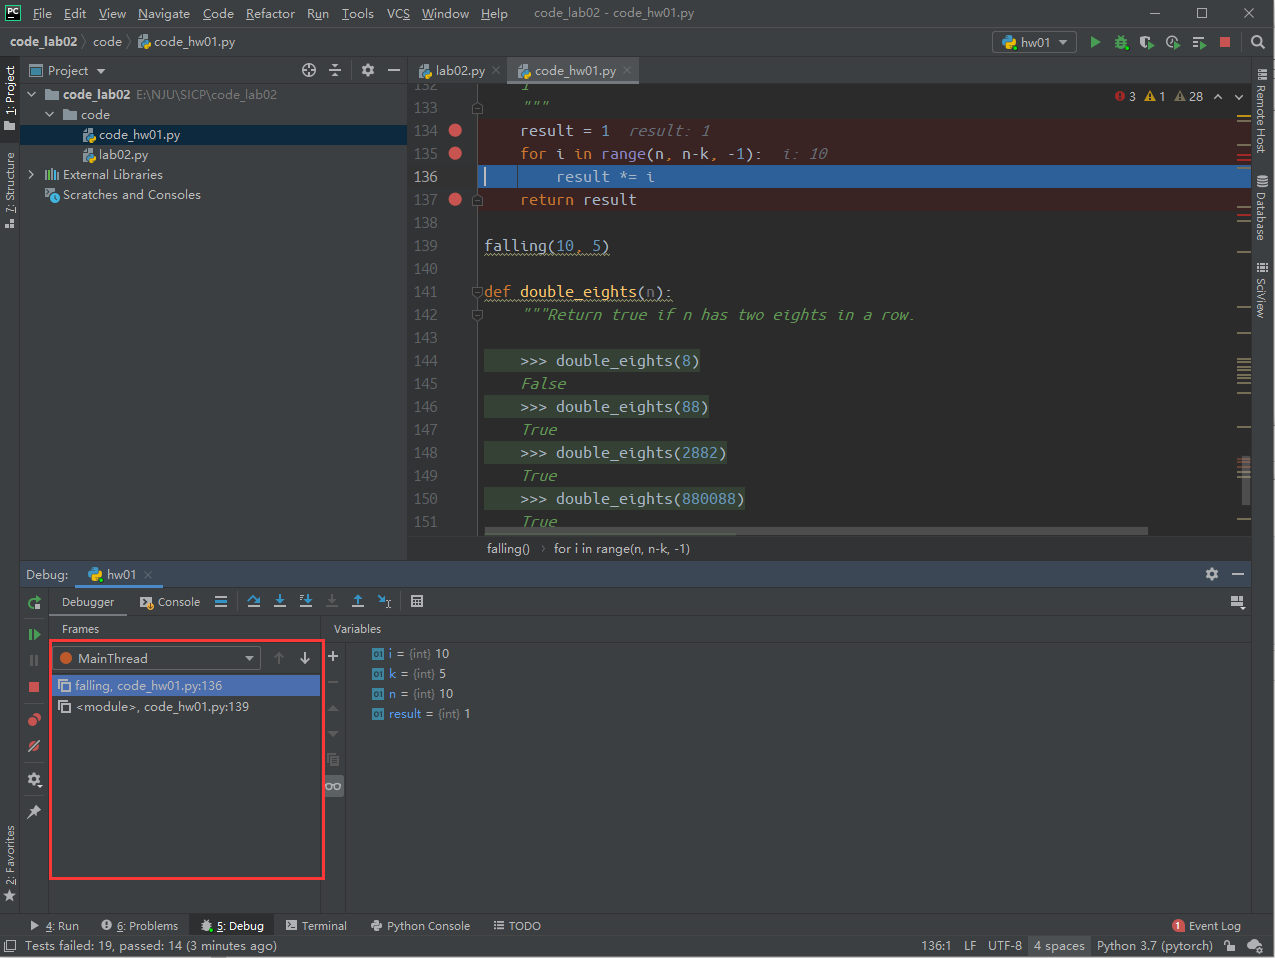
\includegraphics[width=0.5\linewidth]{./imgs/call_stack.png}
    \caption{PyCharm will display call stack in selected regions.}
    \label{fig:breakpoint}
\end{figure}
\vspace{-5mm}
\end{frame}

\begin{frame}
\frametitle{Evaluate Expression}
\begin{figure}
    \centering
    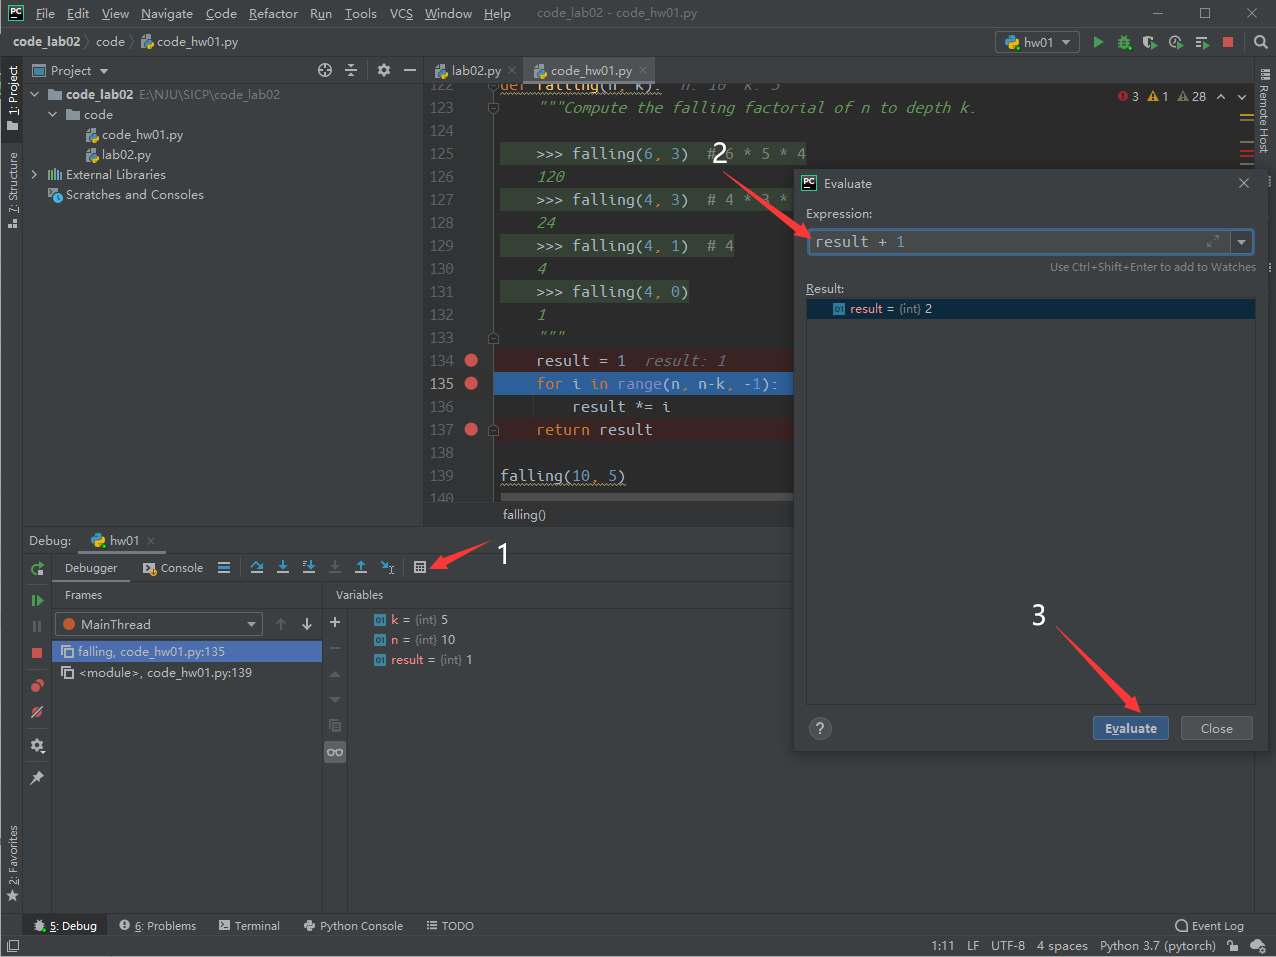
\includegraphics[width=0.5\linewidth]{./imgs/evaluate.png}
    \caption{Evaluate an arbitrary expression.}
    \label{fig:breakpoint}
\end{figure}
\vspace{-5mm}
\end{frame}


\begin{frame}
\frametitle{Run statements}
\vspace{-5mm}
\begin{figure}
    \centering
    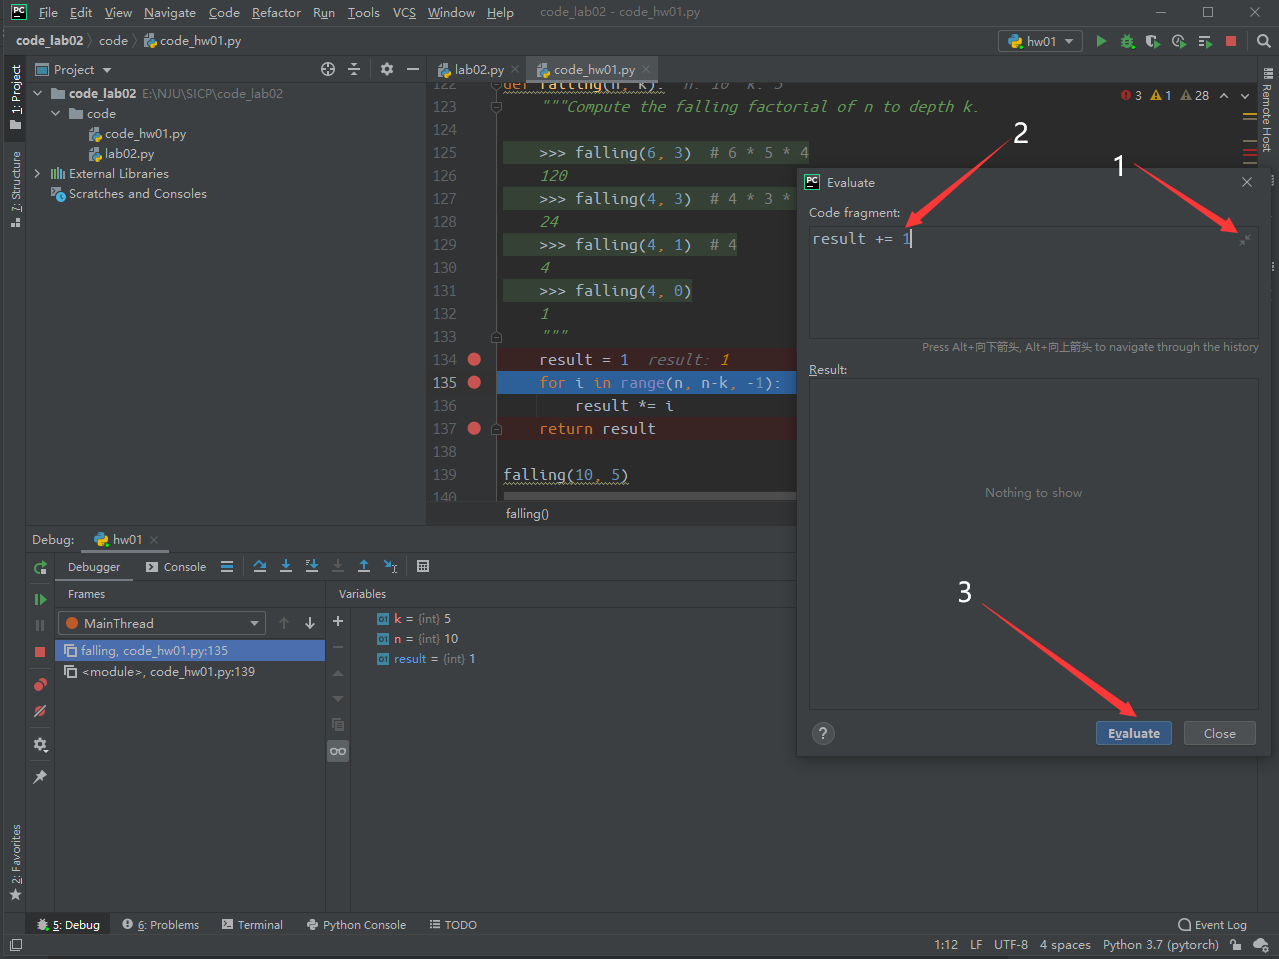
\includegraphics[width=0.4\linewidth]{./imgs/evaluate_2.png}
    \caption{Run arbitrary code.}
    \label{fig:breakpoint}
\end{figure}
\vspace{-5mm}
Note: Statements may change your program frames. For example, if you evaluate \mintinline{text}{result += 1}, \mintinline{text}{result} in your program is bound to \mintinline{text}{2}
\end{frame}

\begin{frame}
\frametitle{Evaluate Expressions and Run Code in Console}

You can also switch to console panel to execute expressions and run code.

\begin{figure}
    \centering
    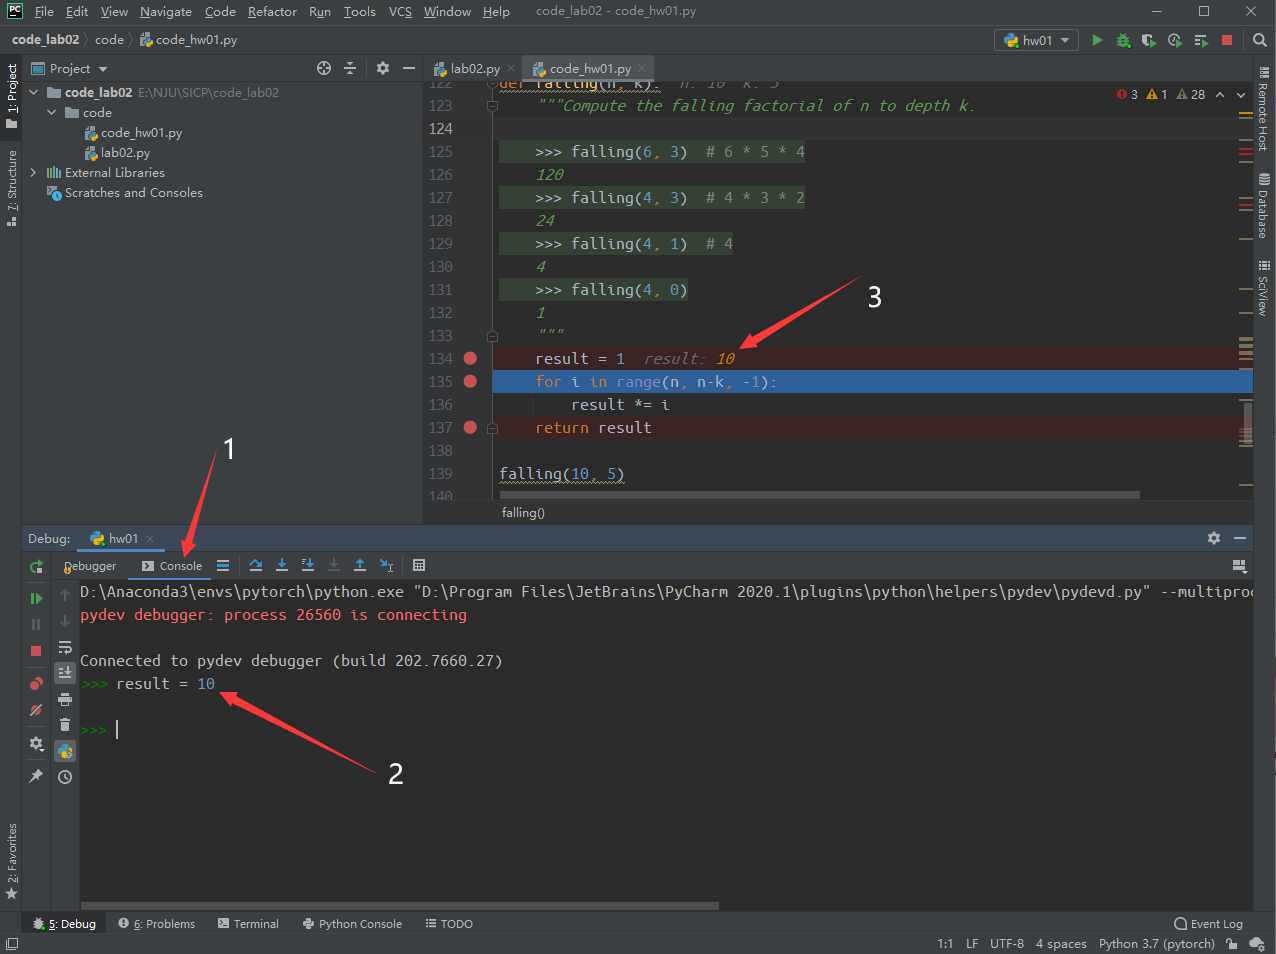
\includegraphics[width=0.5\linewidth]{./imgs/console.png}
    \label{fig:breakpoint}
\end{figure}
\vspace{-5mm}
\end{frame}


\section{Debug using print/assert}
\begin{frame}
\frametitle{Debug using \mintinline{text}{print/assert}}

Debugger is handy. Why bother?

\begin{itemize}
    \item Debugging step by step is too slow;
    \item Programs in debugging mode runs slowly;
    \item Your cannot use a debugger
    \begin{itemize}
        \item Your program is concurrent
        \item Your program runs in a system where no debugger is not supported
    \end{itemize}
    \item You can focus on a specific variable
    \item You do not know how to use a debugger (go back to the Sec~\ref{sec:debugger} and other materials :)
\end{itemize}

\end{frame}

\begin{frame}

\textbf{Main idea}:

Insert \mintinline{text}{print/assert} in your code to see if intermediate results match your expectation.

\end{frame}


\end{document}

\end{document}